\documentclass{article}
\usepackage[margin=1.0in]{geometry}
%\usepackage{amsthm}
\usepackage{hyperref}
\usepackage{alltt}
\usepackage{graphicx}
\usepackage{xcolor}
\usepackage{titling}
\setlength{\droptitle}{-10em}
\raggedbottom
\raggedright
\graphicspath{{}}
\pagecolor[rgb]{0.0, 0.0, 0.0}
\color[rgb]{1, 1, 1}
\title{Data Science Predicts 2023 AMC Profit Margin}
\author{Chris Hamberg}
\date{March, 2023}

\begin{document}
\maketitle{}
\textbf{Results:} 
linear regression analysis was used to predict the future AMC earnings from 
2023 domestic box office projection. The domestic box office is expected to gross
\$9B in 2023. Based off the model, and a \$9B domestic box office, AMC should 
earn approximately -578,841,332 dollars in 2023. There is an approximate 68\%
chance that 2023 earnings will fall within the range of -1,023,877,743 to 
-133,804,920 dollars. There is an approximate 98\% chance that AMC earnings will 
fall within the broader range -1,468,914,155 to 311,231,491 dollars. As an aside,
another model not presented here, but available (see below,) with incredible 
predictive power predicts that AMC needs approximately \$5,643,476,220 in 2023 
revenue to be net profitable. The following binomial function predicts quarterly 
earnings $\hat{y}$ taking quarterly DBO $x$ as it's input:
$$
\hat{y} = f \langle x \rangle 
= -704467565.5695393 + 0.24878099226102765 \cdot x
$$
%\newline \newline
\textbf{More Predictions:} the following table shows predicted yearly earning 
ranges for AMC based on various possible domestic box office numbers (DBO.) All 
numbers in the table are in billions of dollars. "rssd" is the residual squares 
standard deviation $\sigma$. Given quarterly earnings 
$\hat{y} = f \langle x \rangle$ predicted from quarterly DBO $x$, there is an 
approximate 68\% chance that earnings will fall within $\hat{y} \pm \sigma$. For 
that same DBO $x$, there is an approximate 98\% chance that earnings will fall 
within the \hbox{encompassing broader} range of $\hat{y} \pm 2\sigma$. Note that 
displayed values in the table were adjusted from quarterly to yearly outputs.
\newline
\begin{center}
    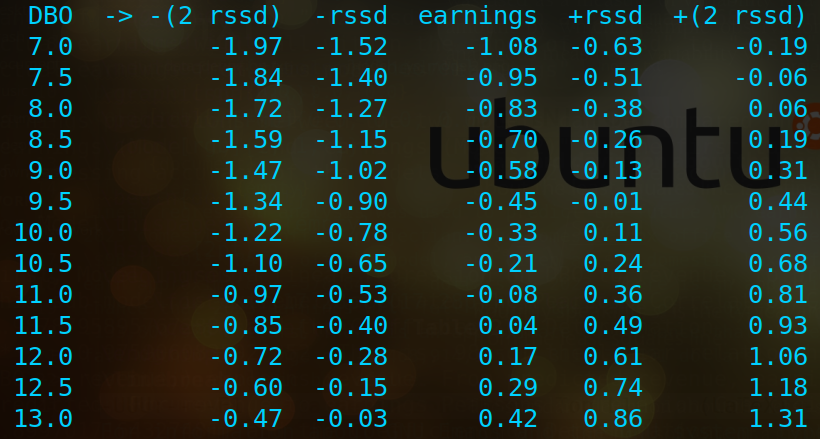
\includegraphics[scale=0.57]{prediction.png}
\end{center}
\vspace{0.2cm}
%\newline \newline
\textbf{About the accuracy of the predictions:}
A strong correlation between DBO and earnings exists such that Pearsons 
Correlation Coefficient is $\approx 0.91$ with the regression line Coefficient of 
Determination $r^{2} \approx 0.82$. Thus, 82\% of the linear relationship 
$(DBO \rightarrow earnings)$ explains earnings. The residual squares standard 
deviation $\sigma$ about the least-squares line is 111,259,102.882163 (x4, to 
convert from quarterly to yearly) compared to the sample standard deviation 
259,856,663.12245965 (x4 to convert from quarterly to yearly.) Thus, the 
regression is a good-fit. The normality test p-value 
$= 9.25190417852916 \cdot 10^{-9}$. This model has incredibly strong predictive 
power. Note that the 2020 Q1 outlier was removed from the dataset.
\newpage
\begin{center}
    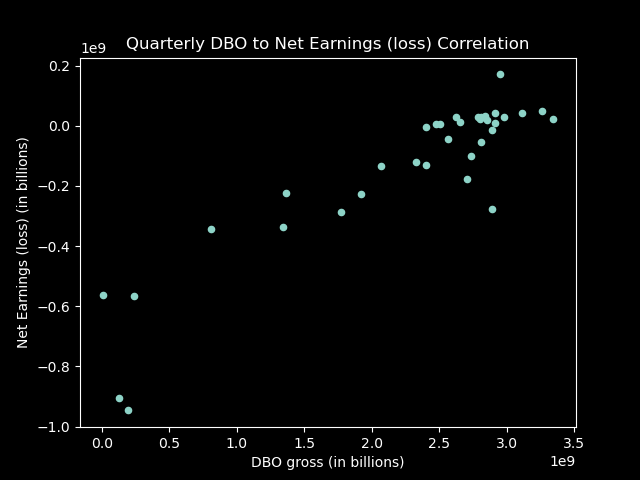
\includegraphics[scale=0.9]{correlation.png}
\end{center}
\begin{center}
    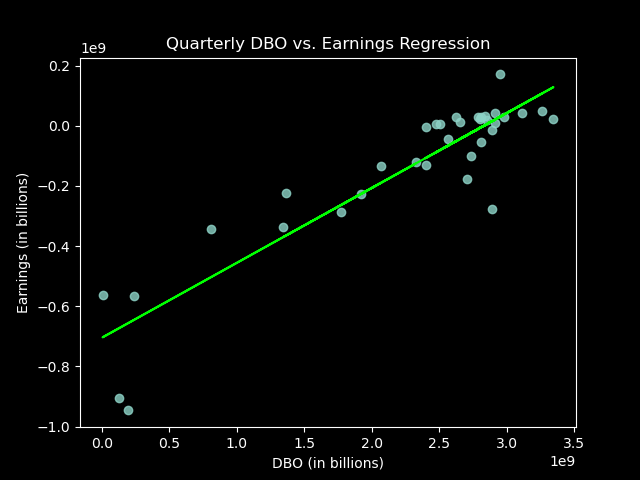
\includegraphics[scale=0.9]{regression.png}
\end{center}
\newpage
\begin{center}
    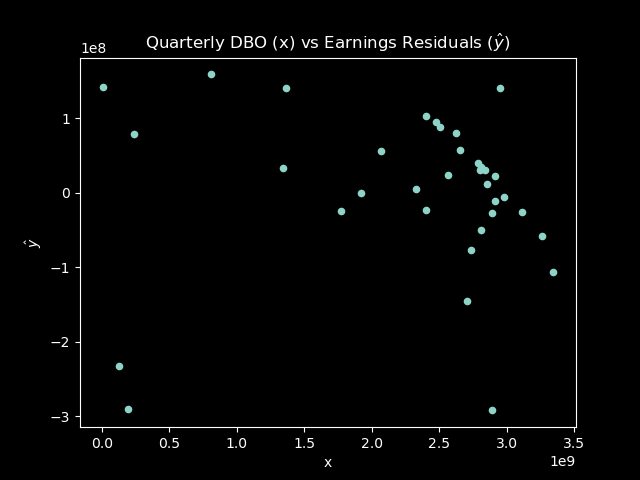
\includegraphics[scale=0.9]{residuals.png}
\end{center}
\textbf{Summary about the Research:} 4 models were constructed to find the best
prediction: 1) predicting earnings from DBO (this model,) 2) predicting revenues  
from DBO, 3) and then predicting earnings from those predicted revenues, and 4) 
estimating revenues from yearly average market share of DBO as the proportion of 
average yearly revenues. Of the 4 models, the one presented is measurably the most 
accurate for predicting earnings, and consists of the greatest predictive power. 
Redundant models were used to cross validate the results. The 4th model was also 
back tested against its historical data. The models, datasets, plots, and this 
document (in PDF format) can be observed and downloaded from the repository: 
\url{github.com/chris-hamberg/fundamentals}
\vspace{1.0cm}
\newline
\textbf{Data Sources:}
\newline \newline
\url{investor.amctheatres.com/financial-performance/}
\newline
\url{boxofficemojo.com/}
\newline
\url{the-numbers.com/market/}
\end{document}